\section{Proposed Method}\label{Sec:Proposal}

In this section, we formalize the task of building confidence regions in the Entropy-Complexity manifold.
Then, we present our proposal to change space through the algorithm of the principal components analysis.
Our goal is to find a latent space representative of the data without the restrictions of the $H\times C$ plane's boundaries.
Through this new representation of the data, we calculate empirical regions with different levels of confidence.
Finally, after calculating these regions, we build a test statistic that determines the probability that a given sequence belongs to the distribution of the points provided.

\subsection{Overall Framework}\label{Sec:OverallFramework}

Our methodology consists of the following steps:
\begin{enumerate}
	\item\label{item:Methodology1} Observe a large number of true random white noise sequences (TRWNS).
	\item\label{item:Methodology2} Map each TRWNS onto a point in the $H\times C$ plane.
	\item\label{item:Methodology3} Obtain the principal components of these points.
	\item\label{item:Methodology4} Compute enclosing boxes in the principal components space.
	\item\label{item:Methodology5} Transform the coordinates of these boxes back to the $H\times C$ plane.
\end{enumerate}

\subsection{True Random Numbers}\label{Sec:TRNG}

Random numbers are used in many fields, from gambling to cryptography, to guarantee a secure, realistic, or unpredictable behavior. 
Pseudorandom results can be achieved by software in a deterministic way, but some applications need actual random numbers (despite the somewhat elusive nature of actual randomness).
Randomness can be observed in unpredictable real-world phenomena like cathodic radiation or atmospheric noise.
%In this study we used two sources of real random numbers. 
%The first is based on vacuum states to generate random quantum numbers described by \citeauthor{RNGVacuumStates}~(\citeyear{RNGVacuumStates}), the second one is based on atmospheric noise captured by a cheap radio receiver presented at \url{www.random.org}.

In this study, we used two sources of true random numbers, both from the observation and measurement of physical phenomena.
The first uses vacuum states. 
The setup consists of an ordinary laser source to generate a local oscillator (LO), a half-wave plate, a polarizing beamsplitter (BPS), and two balanced detectors working together adding or subtracting the photocurrents results in a quadrature measurement of the LO or vacuum state. 
The distribution of the vacuum state is binned into $2^n$ equal parts (bins of the same size), assigning a fixed bit combination of length $n$ to each sample point in a given bin \citep{RNGVacuumStates}. 
The second one employs atmospheric noise captured by a cheap radio receiver with no filter for unwanted static sounds caused by atmospheric noise.
This generator was implemented over a distributed setup with radios located at different geographical locations sending random bits to a cloud server that processes data and hosts the values.
The history of this service and other information can be found at \citet{RandomOrg}.

We used \SI{54e6}{4\byte} words from each physical generator, which approximately amounts \SI{200}{\mega\byte} of data.

%\textcolor{red}{Fornecer mais informações. Quantos dados em bits, ou bytes, ou outra unidade, foram empregados de cada fonte, e como foram armazenados. Precisão simples, certo?}

\subsection{Parameters Settings and Dataset}\label{Sec:Parameters}

We conducted an ablation study to identify the influence of the parameters $T$, $D$, and $\tau$ in the construction of empirical confidence regions.
We verified that the results involving the time delay parameter variation did not show significant differences in repeated experiments; therefore, in the sequel, we did no consider $\tau$ as a determining factor.
On the other hand, we found two relevant variables: 
the length of the sequence 
and the embedding dimension.
We, thus, employed the following factors:
\begin{itemize}
	\item Sequence length $T\in\mathcal T=\{ \num[scientific-notation=true]{e3}, \num[scientific-notation=true]{5 e4}\}$,
	\item Embedding dimension $D\in\mathcal D=\{3, 4, 5, 6\}$.
	%,and
	%\item Time delay $\tau=\{1, 10, 30, 50\}$.
\end{itemize}
and kept $\tau=1$, which is the most frequently used option.
The values of $D$ are within the range recommended in the literature~\citep{PermutationEntropyBandtPompe}.

Using this parametric space, we analyzed the different degrees of information captured by the ordinal patterns formed.
For the construction of the confidence regions presented, we used:
\begin{itemize}
	\item A set of \num{104596} points in the $H \times C$ plane, corresponding to sequences of length $T = 1000$, for each value of $D\in \mathcal D$, and
	\item  a set of \num{2093} points in the $H \times C$ plane, corresponding to sequences of length $T = 50000$, for each value of $D \in \mathcal D$.
\end{itemize}

We used the \texttt R platform \citep[][v.~4.0.3]{Rmanual} for data generation and analyses, and the \texttt{ggplot2} library \cite{ggplot2Wickman} for generating the plots.

\begin{comment}

\begin{figure}
\centering
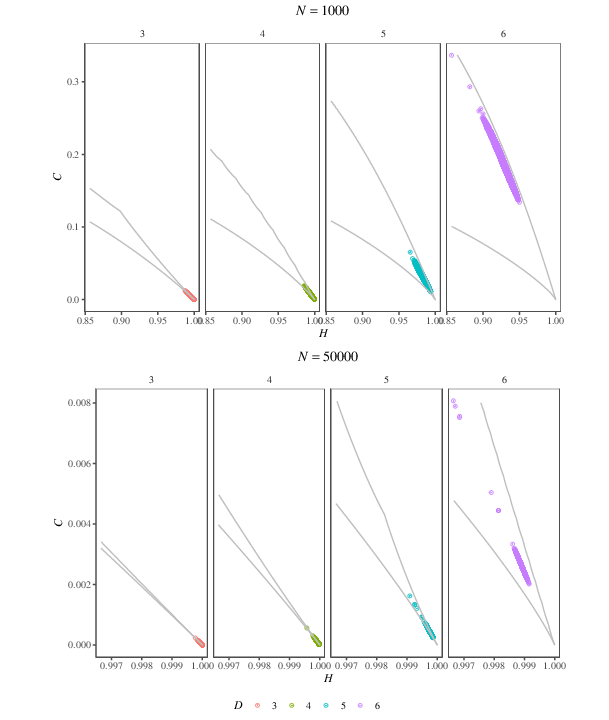
\includegraphics[width=\linewidth]{Figures/Points-PDF.png}
\caption{White noise samples considered during the construction of the proposed confidence regions.}
\label{fig:white-noise}
\end{figure}

\end{comment}

\subsection{Empirical Confidence Regions and $p$-values}\label{confidenceRegions}

%As we do not know the joint probability distribution of the pair $(h, c)$ for a sequence of random variables collectively independent and identically distributed according to a uniform law, studies involving classical bi-variate analysis, linear regression, and generalized linear models become unfeasible.

Our first approaches to analyzing sequences of points in the $H\times C$ plane produced by TRWNS verified that they, and usual transformations, are far from bivariate Gaussian and generalized Hyperbolic distributions \Mycite{MultivariateDistributionModelswithGeneralizedHyperbolicMargins}.
Different types of regression models of $C$ explained by $H$ did not produce acceptable results.
Thus, we adopted a non-parametric approach and made an empirical analysis of the data obtained from physical sources for using them as our reference in the search for confidence regions and $p$-values.
%Therefore, for the construction of our proposal, we adopted a non-parametric approach, making an empirical analysis of data obtained from physical sources and using them as our reference in the search for confidence regions.

%The set of all feasible pairs in the $H \times C$ plane is found in a compact subset of $\mathbbm{R}^2$, which has limits with explicit expressions for the boundaries of this closed manifold, dependent only on the dimension of the probability space considered, that is $D!$ in the traditional Bandt-Pompe method~\citep{martin2006generalized}.
%Due to such quotas, some limitations are generated, such as the absence of a representative distance metric and the difficulty of proposing confidence regions.
%In view of this, it is necessary to apply an orthogonal projection in the data for a new two-dimensional coordinate system to solve these restrictions.
%A classic proposal in these categories of problems is the principal component analysis algorithm~\citep{wold1987principal}.

Let $\utilde{x} =(x_1, x_2, \dots, x_N)$ be $N$ times series of length $T$, and define an embedding dimension $D$.
In the sequel, whenever possible, we will omit $T$ and $D$.
For each $n=1,2,\dots, N$, the time series $x_n$ is mapped onto the point $(h_n,c_n)$ in the $H\times C$ plane, thus $\utilde{hc}=\big((h_1,c_n), (h_2,c_2), \dots, (h_N,c_N)\big)$ are the points that correspond to the $N$ time series.
Fig.~\ref{fig:Methodology1} illustrates this step.
We will obtain confidence regions and $p$-values from $\utilde{hc}$.

The first step consists in finding and applying the principal components transformation to $\utilde{hc}$.
With this, we obtain the set of uncorrelated points $\utilde{uv}=\big((u_1,v_1), (u_2,v_2),\dots,(u_N,v_N)\big)$, in which $u_n$ and $v_n$ are the first and second principal components of $h_n$ and $v_n$, respectively.
This projection allows us to obtain a ``central'' point of the data set, around which we will build a rectangular box containing \SI{100}{\minusalphapercent} of the observations.
Such box is a variation of the bagplot \citep{TheBagplotaBivariateBoxplot}.
Notice that finding the smallest box that encloses $k$ out of $N$ points is difficult; cf.\ the work by \citet{SmallestKEnclosingRectangleRevisited}.

For simplicity, and without loss of generality, assume $N$ is odd.
\begin{enumerate}
	\item Find the indexes that sort the values of the first principal component $\bm u=(u_1,u_2,\dots,u_N)$ in ascending order: $\bm r=(r_1,r_2,\dots,r_N)$, i.e., $u_{r_1}$ is the minimum value, and $u_{r_N}$ is the maximum value.
	\item\label{item:Median} Find the point $(u,v)$ whose first principal component is the median: $(u_{r_{(N+1)/2}}, \cdot)$. Apply the inverse principal components transformation, and obtain $\bm P'=(h',v')$. Call the corresponding time series ``emblematic time series.''
	\item\label{item:Point1} Find the point $(u,v)$ whose first principal component is the quantile $\alpha/2$: $(u_{r_{[N\alpha/2]}}, \cdot)$.
	\item\label{item:Point2} Find the point $(u,v)$ whose first principal component is the quantile $1-\alpha/2$: $(u_{r_{[N(1-\alpha/2)]}}, \cdot)$.
	\item\label{item:Point3} The values $u_{r_{[N\alpha/2]}}$ and $u_{r_{[N(1-\alpha/2)]}}$ are the rightmost and leftmost bounds of the box, respectively.
	\item\label{item:Point4} The bottom bound of the box is the smallest second principal component value whose first principal component is at least $u_{r_{[N\alpha/2]}}$; denote this values $v_{\min}$.
	\item\label{item:Point5} The top bound of the box is the largest second principal value whose first principal component is at most $u_{r_{[N(1-\alpha/2)]}}$; denote this value $v_{\max}$.
	\item The corners of the box are 
	$(u_{r_{[N\alpha/2]}}, v_{\min})$, 
	$(u_{r_{[N\alpha/2]}}, v_{\max})$, 
	$(u_{r_{[N(1-\alpha/2)]}}, v_{\min})$ and 
	$(u_{r_{[N(1-\alpha/2)]}},v_{\max})$.
	\item\label{item:BoxHxC} Apply the inverse principal components transformation to these corners obtaining $\bm P_1=(h_{v_1}, c_{v_1})$, $\bm P_2=(h_{v_2},h_{v_2})$, $\bm P_3=(h_{v_3}, c_{v_3})$ and $\bm P_4=(h_{v_4},c_{v_4})$.
\end{enumerate}

Fig.~\ref{fig:methodology} illustrates these steps.
%
Fig.~\ref{fig:Methodology1} shows the points produced by TRWNS in the $H\times C$ plane.
The blue box includes a certain percentage of points, with sides parallel to the $H$ and $C$ axes.
The area in the $H\times C$ plane overestimates the desired proportion and may include ``unacceptable'' points.
%
Fig.~\ref{fig:Methodology2} shows the previous points projected onto the principal components space (steps~\ref{item:Median} to~\ref{item:Point5}).
The red box includes the same percentage of desired points, with axes parallel to the first and second principal components.
We highlighted in red the point whose first principal component is the median of the observed values.
%
Fig.~\ref{fig:Methodology3} shows the result of projecting back the red box from the principal components space to the $H\times C$ plane (step~\ref{item:BoxHxC}).
The comparison of the red and blue boxes shows that the area has been reduced, thus improving the test's power.

\begin{figure}[hbt]
	\centering
	%    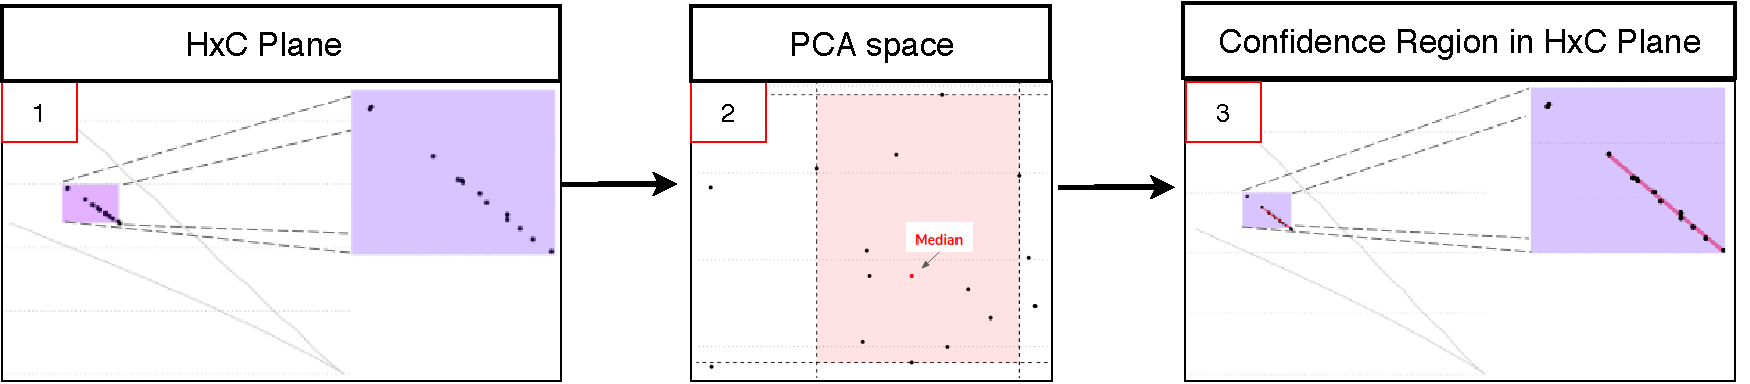
\includegraphics[width=\linewidth]{Figures/Methodology.pdf}
	\subfloat[Mapping true white noise random sequences onto the $H\times C$ plane.\label{fig:Methodology1}]{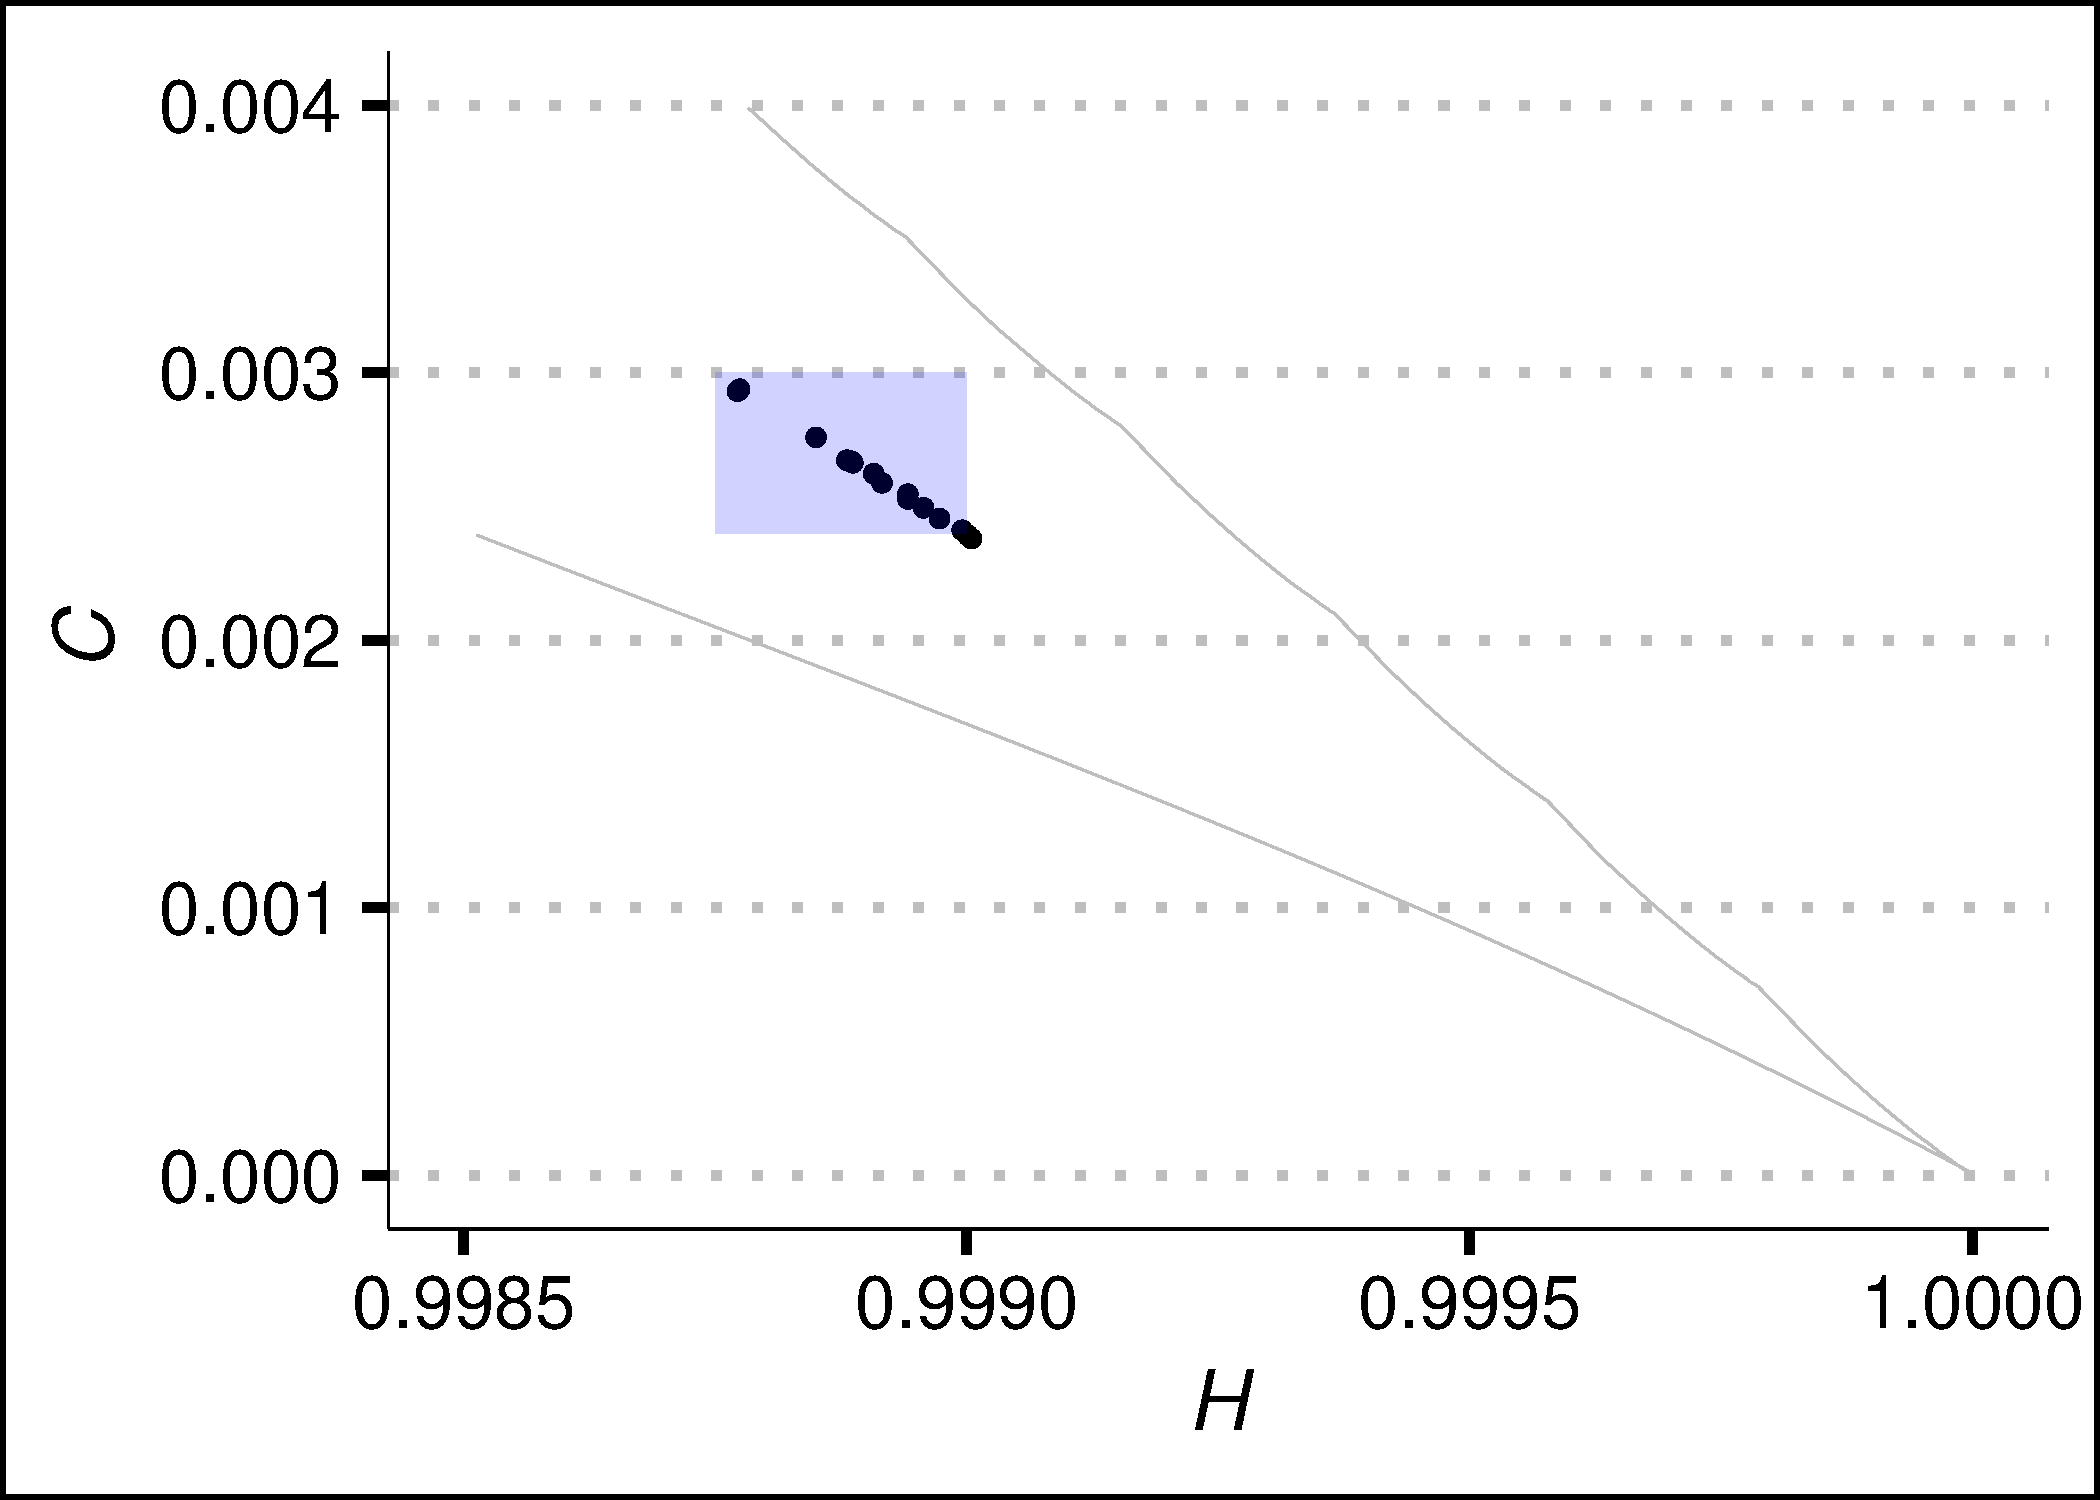
\includegraphics[width=.33\linewidth]{step1}}
	\subfloat[Transformation of the points in the $H\times C$ plane by Principal Components, and determination of minimal boxes.\label{fig:Methodology2}]{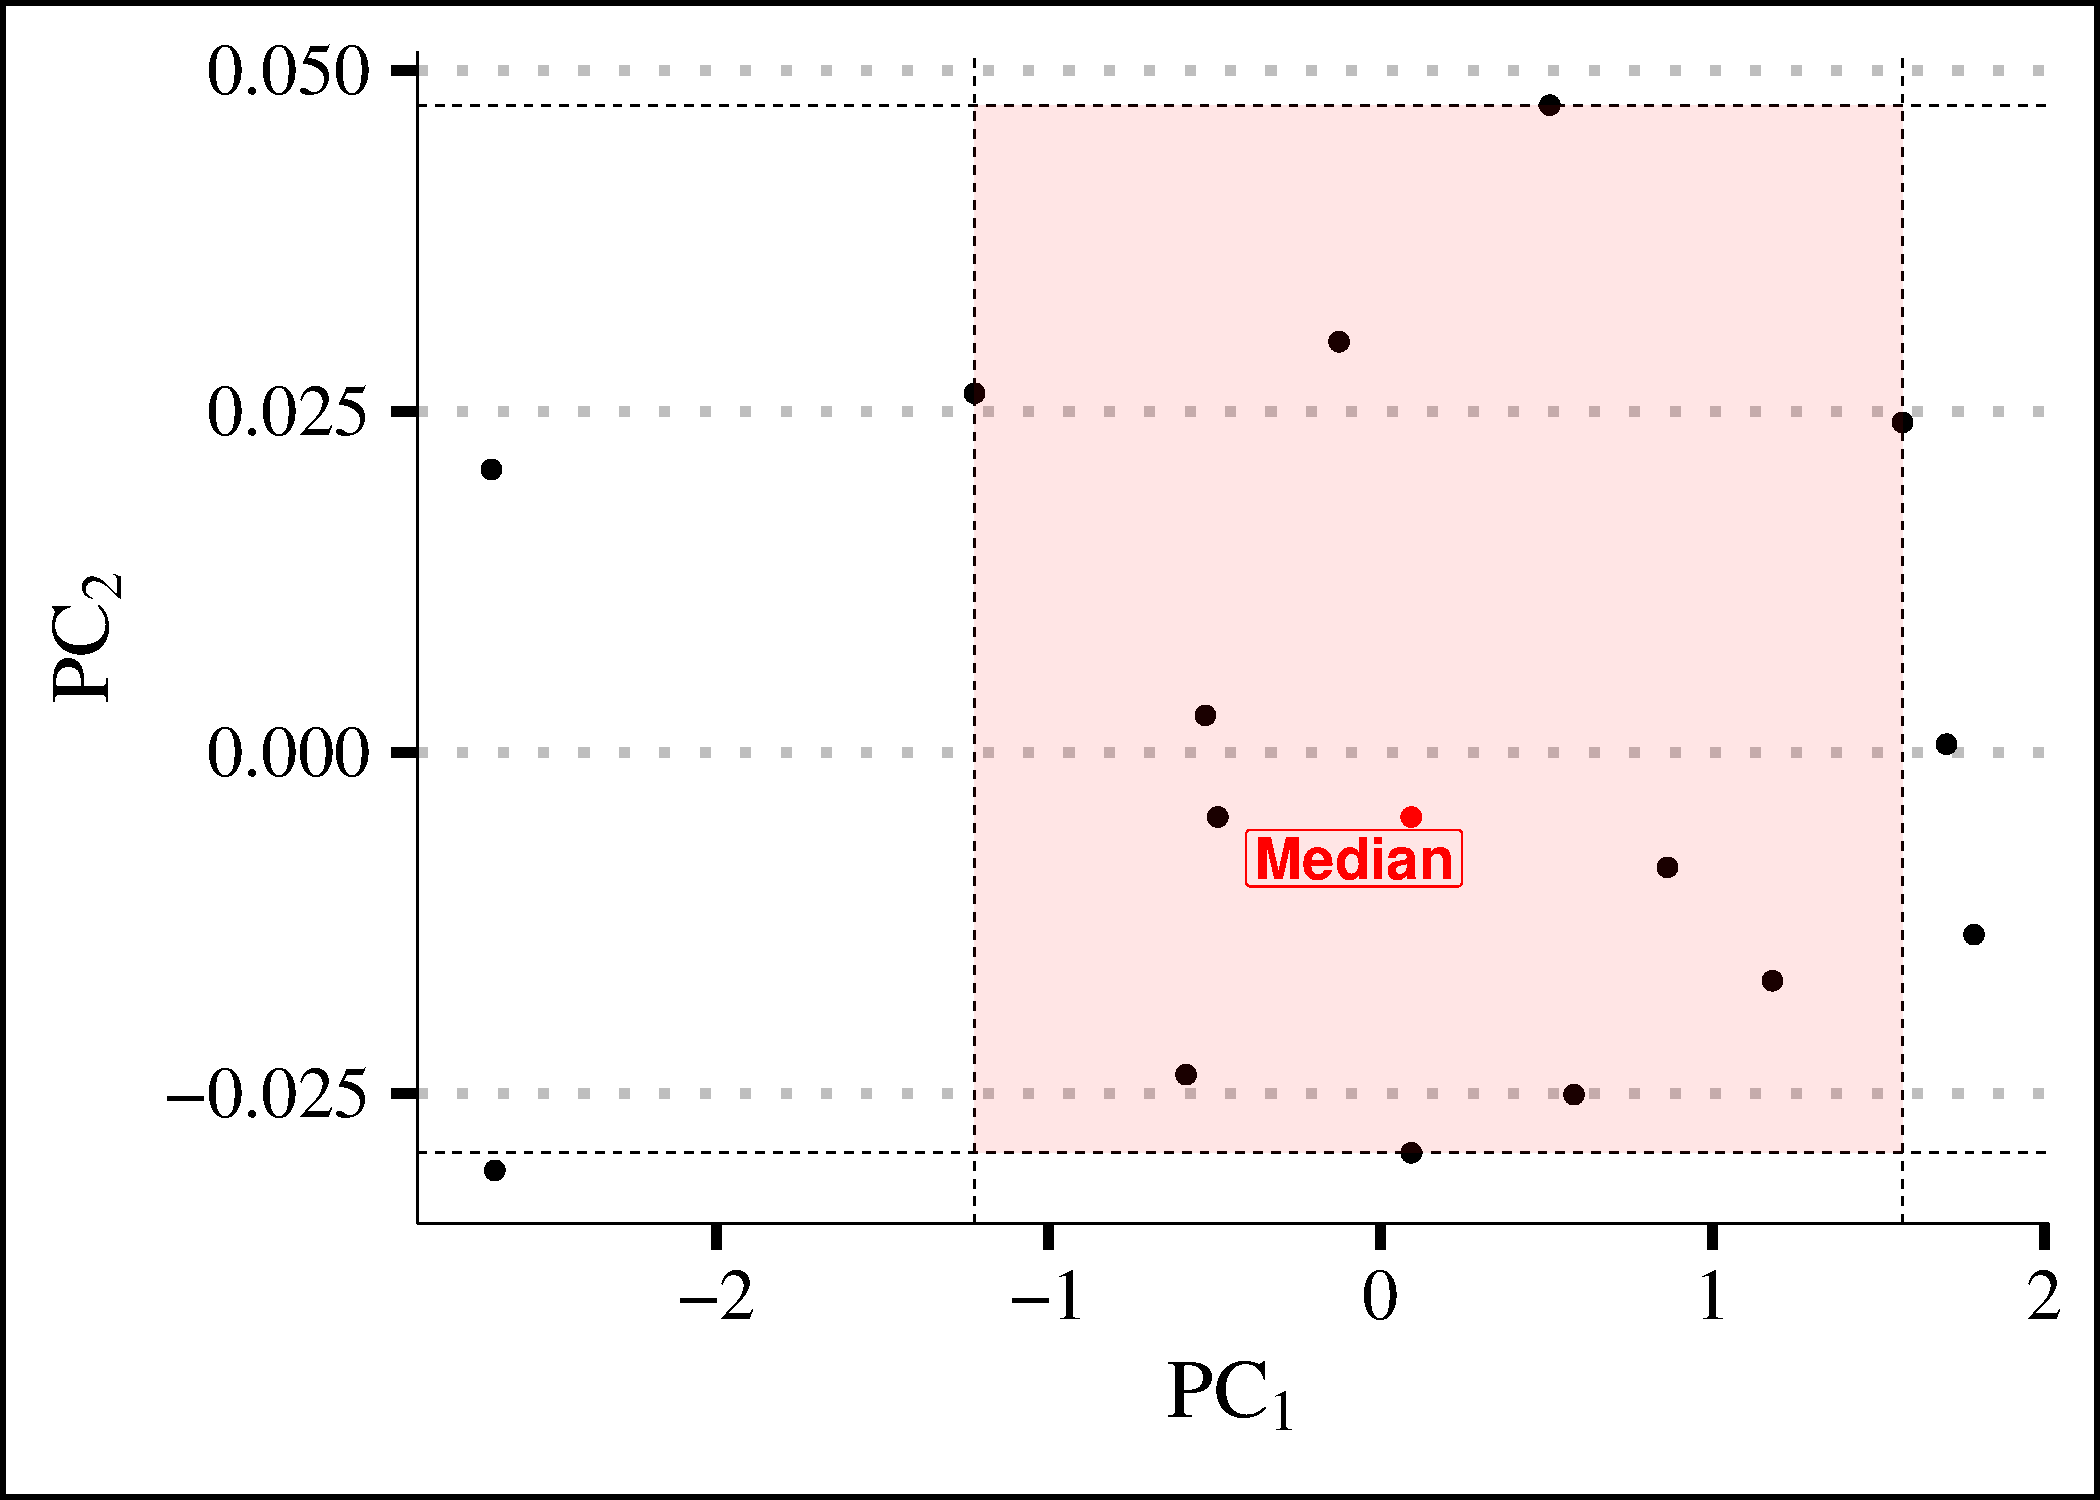
\includegraphics[width=.33\linewidth]{step2}}
	\subfloat[Inverse transformation from the Principal Components plane to the $H\times C$ plane.\label{fig:Methodology3}]{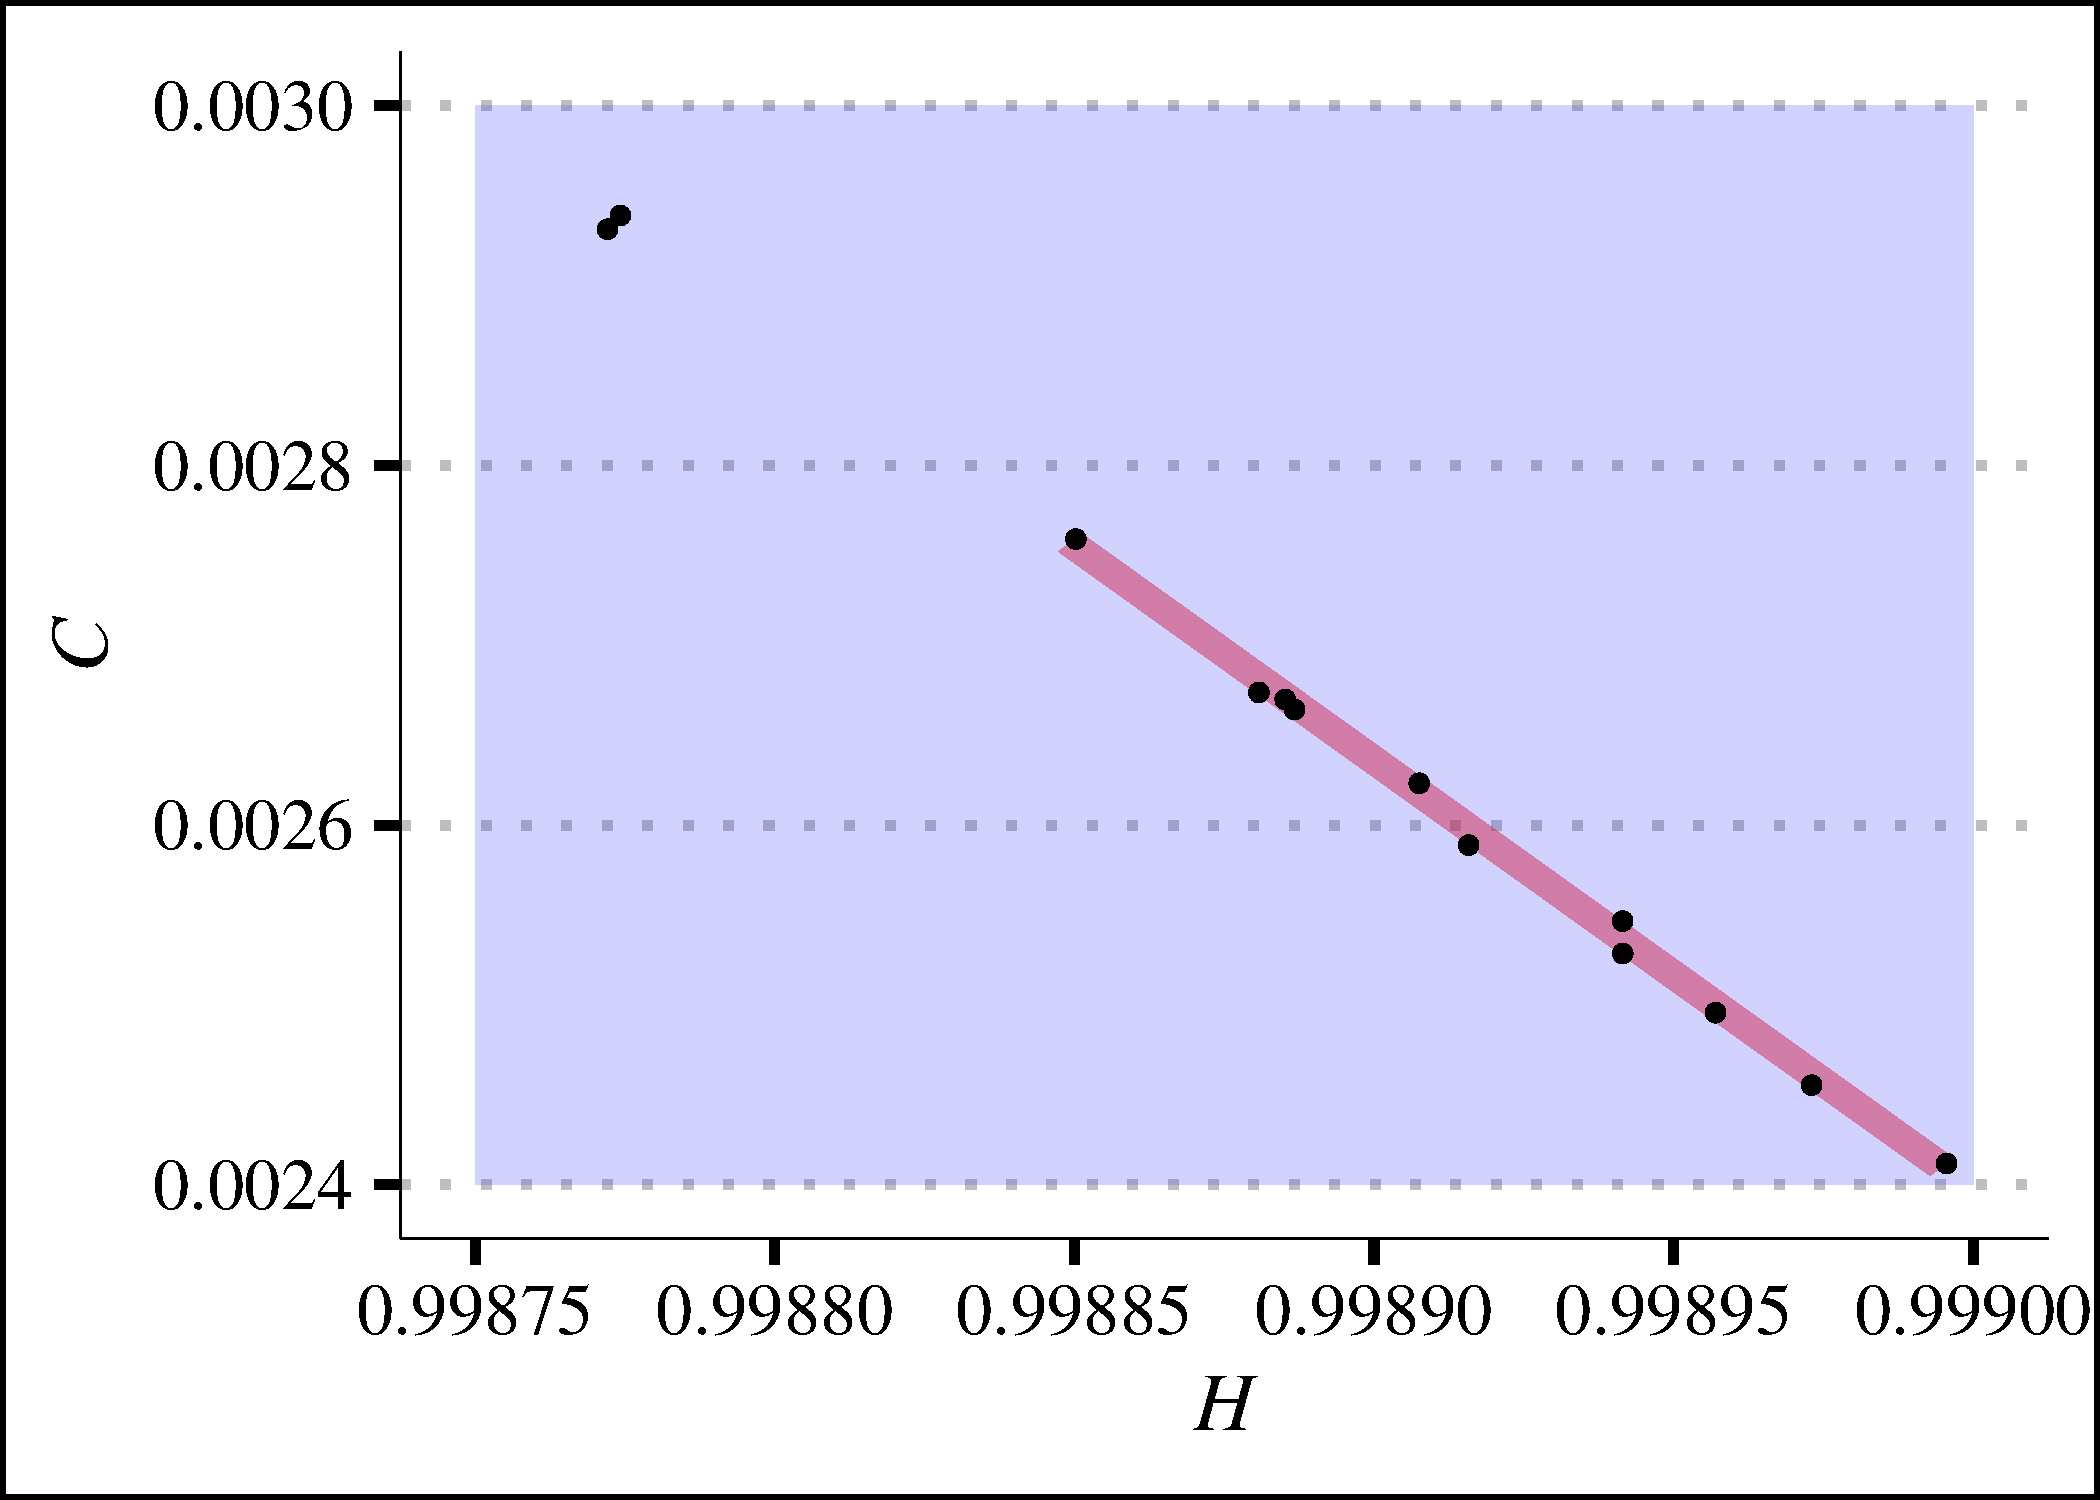
\includegraphics[width=.33\linewidth]{step3}}
	\caption{Outline of the methodology used for the construction of the confidence regions.}
	\label{fig:methodology}
\end{figure}

Algorithm~\ref{Algo:ConfidenceRegions} provides details on how we obtain the confidence regions, defined by a set of points $\bm P_1, \bm P_2, \bm P_2, \bm P_4$, for each $D\in \mathcal D$, each $T\in \mathcal T$, and each significance level $\alpha$.
We also obtain the ``emblematic point'' $\bm P'$, a kind of median point in the $H\times C$ plane for each situation.


\begin{algorithm}[hbt]
	\SetKwInOut{Input}{input}\SetKwInOut{Output}{output}
	\Input{A data base of true random values}
	\Input{The desired values of embedding dimension $\mathcal D$, sequence length $\mathcal T$, and confidence levels $\mathcal A$}
	\Output{Confidence regions as points in the $H\times C$ plane}
	\For{each $D\in \mathcal D$}{
		\For{each $T\in \mathcal T$}{
			\For{each $n=1,2,\dots,N$}{
				build the time series $p_n$ with unused values from the data base\;
				compute the point $(h_n,c_n)$ in the $H\times C$ plane that corresponds to $p_n$\; 
			}
			obtain $\text{PC}(D,T)$, the principal components transformation based on the points $(h_1,c_1),(h_2,c_2),\dots,(h_N,c_N)$, and its inverse $\text{PC}^{-1}(D,T)$\;
			%
			apply $\text{PC}(D,T)$ to the points $(h_1,c_1),(h_2,c_2),\dots,(h_N,c_N)$, and obtain $(u_1,v_1),(u_2,v_2),\dots,(u_N,v_N)$\;
			%
			find the indexes $\bm r=(r_1,r_2,\dots,r_N)$ that sort the values of the first principal component $\bm u=(u_1,u_2,\dots,u_N)$ in ascending order\;
			%
			find the point $(u,v)$ whose first principal component is the median: $(u_{r_{(N+1)/2}}, \cdot)$\;
			%
			apply the inverse principal components transformation $\text{PC}^{-1}(D,T)$ to $(u,v)$, and obtain $\bm P'=(h',v')$; call the corresponding time series ``emblematic time series''\;
			\Return{$\bm P'$}\;
			%
			\For{each confidence level $\alpha \in \mathcal A$}{
				find the point $(u,v)$ whose first principal component is the quantile $\alpha/2$: $(u_{r_{[N\alpha/2]}}, \cdot)$\;
				%
				find the point $(u,v)$ whose first principal component is the quantile $1-\alpha/2$: $(u_{r_{[N(1-\alpha/2)]}}, \cdot)$\;
				%
				the values $u_{r_{[N\alpha/2]}}$ and $u_{r_{[N(1-\alpha/2)]}}$ are the rightmost and leftmost bounds of the box, respectively\;
				%
				the bottom bound of the box is the smallest second principal component value whose first principal component is at least $u_{r_{[N\alpha/2]}}$; denote this value $v_{\min}$\;
				%
				the top bound of the box is the largest second principal value whose first principal component is at most $u_{r_{[N(1-\alpha/2)]}}$; denote this value $v_{\max}$\;
				%
				the corners of the box are 
				$(u_{r_{[N\alpha/2]}}, v_{\min})$, 
				$(u_{r_{[N\alpha/2]}}, v_{\max})$, 
				$(u_{r_{[N(1-\alpha/2)]}}, v_{\min})$ and 
				$(u_{r_{[N(1-\alpha/2)]}},v_{\max})$\;
				%
				apply the inverse principal components transformation $\text{PC}^{-1}(D,T)$ to these corners obtaining $\bm P_1=(h_{v_1}, c_{v_1})$, $\bm P_2=(h_{v_2},h_{v_2})$, $\bm P_3=(h_{v_3}, c_{v_3})$ and $\bm P_4=(h_{v_4},c_{v_4})$\;
				\Return{$\bm P_1$, $\bm P_2$, $\bm P_3$, $\bm P_4$}\;
			}
		}
	}
	\caption{Determination of confidence regions and emblematic time series}\label{Algo:ConfidenceRegions}
\end{algorithm}


%The visual representation of the proposed technique can be seen in Fig.~\ref{fig:methodology}.

These confidence regions obtained provide a powerful tool to make binary assessments about the adequacy of a given time series $\bm x$ to the null hypothesis $\mathcal H_0$ that it is white noise.
More generally, we are interested in obtaining the $p$-value of $\bm x$ under $\mathcal H_0$.
We present a procedure to obtain an approximate $p$-value based on the evidence collected to build the confidence regions.

The procedure operates on the principal components space and consists of measuring the closeness between the ``emblematic point'' and the observed point.
We are given a time series $\bm x$ of size $T$, and we want its $p$-value when contrasted with TWNRS of the same size at embedding dimension $D$.
We use $N$ TWNRS of size $T$, compute their points in the $H\times C$ plane, and project them to the corresponding principal components space.
We then do the same with $\bm x$, and obtain a new point $(u_x,v_x)$.
The closer $\bm x$ is to the emblematic time series, the larger its $p$-value.
Assume that the emblematic time series is represented by $(u,v)$ in the principal components space.
We measure this closeness by building a box around $(u_x,v_x)$ that contains $(u,v)$; assume that $u_x>u$, then:
\begin{enumerate}
	\item the right side of the box is the smallest $u_j$ which is larger that $u_x$; assume it corresponds to the quantile $\eta_u$ of $\utilde u = (u_1,u_2,\dots, u_N)$. By definition, $\eta_u\geq 1/2$.
	%
	\item the left side of the box is the $1-\eta_u$ quantile of $\utilde u$.
	%
	\item the top side of the box is the smallest $v_j$ which is larger that $v_x$; assume it corresponds to the quantile $\eta_v$ of $\utilde v = (v_1,v_2,\dots, v_N)$. By definition, $\eta_v\geq 1/2$.
	%
	\item the bottom side of the box is the $1-\eta_v$ quantile of $\utilde v$.
\end{enumerate}
Fig.~\ref{fig:methodologyPvalue} illustrates theses steps.

The definition of the box for the case $u_x<u$ follows naturally, and is described in Algorithm~\ref{Algo:p-value}.
With this approach, we obtain the smallest box that (i)~contains the new point, and (ii)~is defined by observed points from TRWNS.

Such boxes are less prone to distortions in this space since the distribution of the points becomes less asymmetric than in the $H\times C$ plane; cf.\ Fig.~\ref{fig:HC-PCA}.
Algorithm~\ref{Algo:p-value} shows the details.

\begin{figure}[hbt]
	\centering
	\subfloat[Points produced by TRWNSs in the space of principal components.\label{fig:v1}]{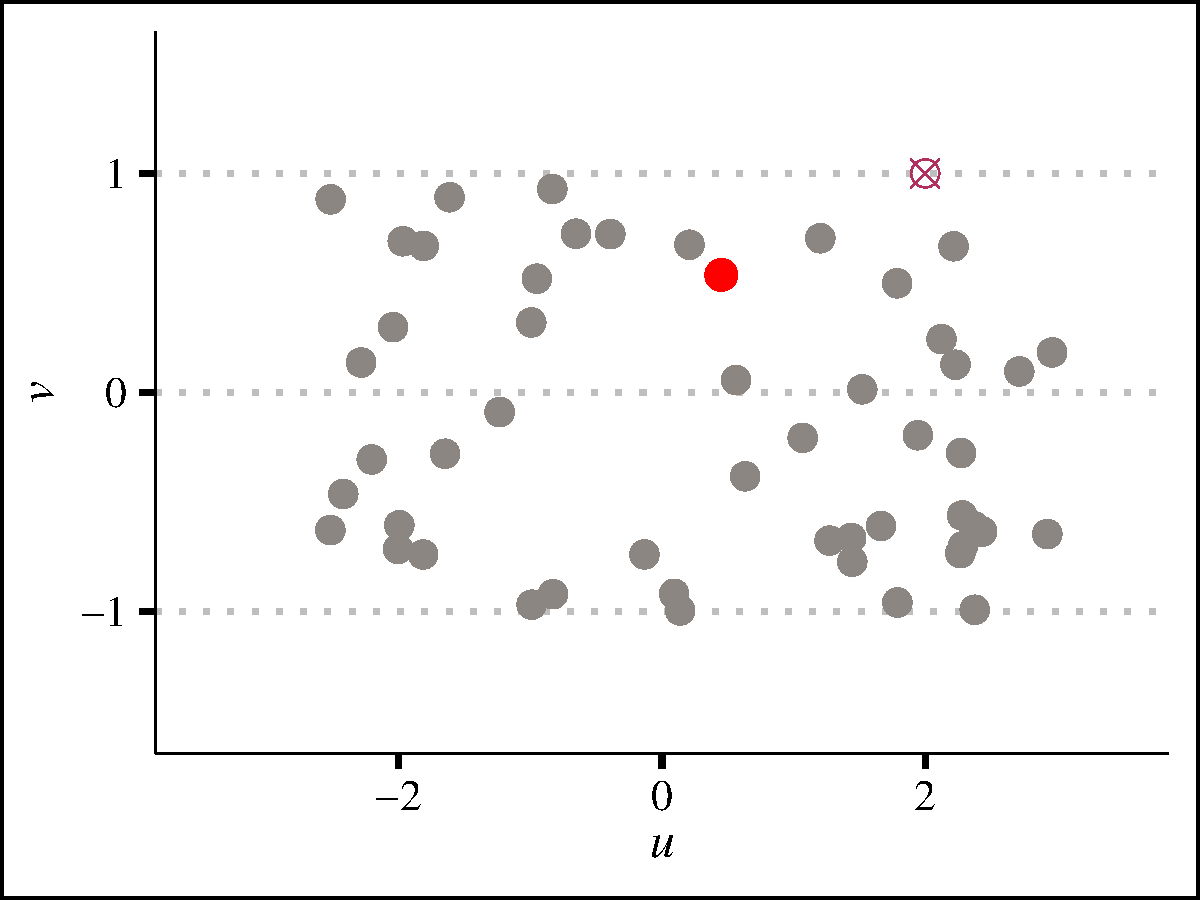
\includegraphics[width=.33\linewidth]{PvalueStep1}}
	\subfloat[Points whose first principal component is the median (red) and quantiles of order $\eta_u$ and $1-\eta_u$ (green).\label{fig:methodologyPvalue2}]{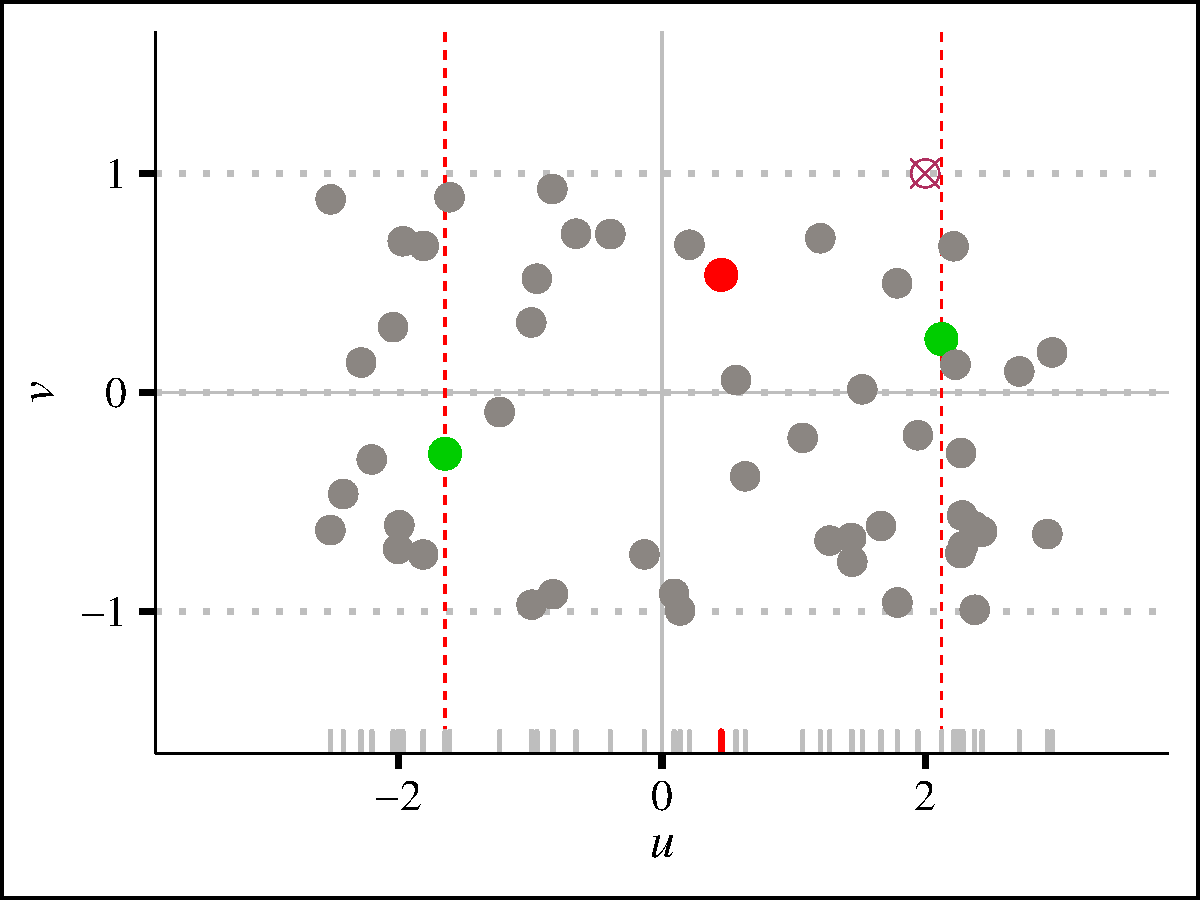
\includegraphics[width=.33\linewidth]{PvalueStep2}}
	\subfloat[The $p$-value of the new point is the proportion of points outside the box.\label{fig:methodologyPvalue3}]{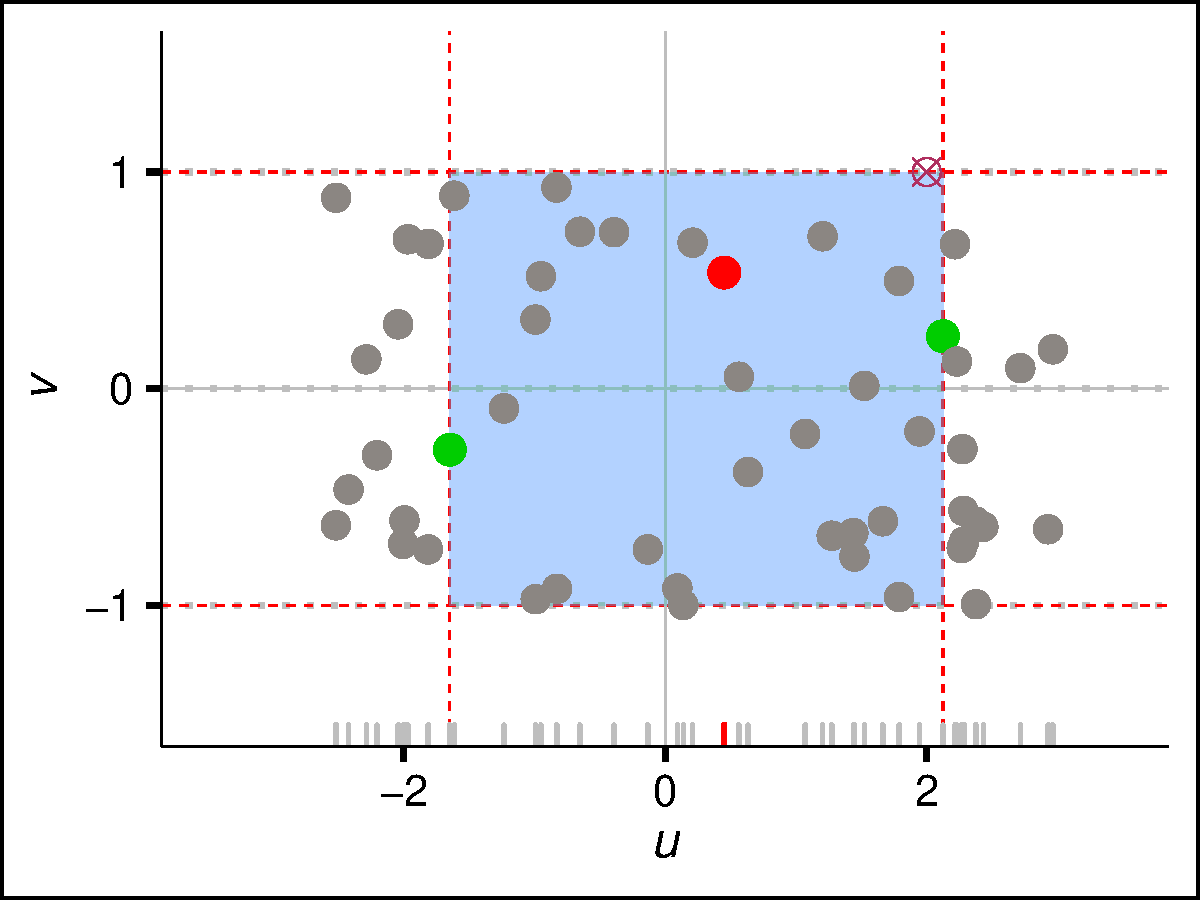
\includegraphics[width=.33\linewidth]{PvalueStep3}}
	\caption{Outline of the methodology used to calculate the $p$-value. The new point is denoted as a crossed circle.}
	\label{fig:methodologyPvalue}
\end{figure}

\begin{comment}
The empirical $p$-value of $\bm x'$ for the null hypothesis is given by the percentage of points outside the lowest confidence region obtained by the reference points to which $\bm x'$ belongs.
Therefore, it can be achieved by the following steps:
\begin{enumerate}
\item Compute $(h',c')$ the point in the $H\times C$ plane produced by $\bm x'$;
\item Compute $b_{T,D}(\bm x')$: the smallest box which contains $(h',c')$ using the $M$ reference points;
\item The empirical $p$-value of $\bm x'$ is obtained by the percentage of reference points outside $b_{T,D}(\bm x')$.
\end{enumerate}
Thus, we can verify that:
\begin{itemize}
\item the smallest $b_{T,D}(\bm x')$ is observed when $(h',c')$ ``coincides'' with the point produced by the emblematic sequence, in other words, point whose first principal component is the median of the $M$ reference points, and
\item the largest box is any box associated to $(h',c')$ ``outside'' the largest box produced by the $M$ reference points.
\end{itemize}
Assuming the critical value $\alpha = 0.05$, we obtain:
\begin{equation*}
p-\text{value} \geq \alpha, \text{ the null hypothesis should not be rejected}.
\end{equation*}
\end{comment}

\begin{algorithm}[hbt]
	\SetKwInOut{Input}{input}\SetKwInOut{Output}{output}
	\Input{The sequence $\bm x$ of length $T$ to be contrasted to the null hypothesis $\mathcal H_0$ that it is adherent to white noise}
	\Input{The embedding dimension $D$}
	\Input{$N$ points $(h_1,c_1),(h_2,c_2),\dots,(h_N,c_N)$ of true white noise series of length $T$;
		the principal components tranformation $\text{PC}(D,T)$ induced by these points;	
		the points projected onto the $H\times C$ plane: $(u_1,v_1),(u_2,v_2),\dots,(u_N,v_N)$}
	\Output{An approximate $p$-value}
	find the point $(u,v)$ whose first principal component is the median: $(u_{r_{(N+1)/2}}, \cdot)$\;
	find the point $(h,c)$ of the sequence $\bm x$\;
	find the projection $(u_x,v_x)$ of $(h,c)$ onto the principal components space using $\text{PC}(D,T)$\;	
	\eIf{$u_x > u$}
	{ $u_{r_{[N(1-\alpha/2)]}}$ is defined as the smallest element larger than $u_x$\;
		$u_{r_{[N\alpha/2]}} \leftarrow 2u - u_{r_{[N(1-\alpha/2)]}}$\;
	}
	{
		\eIf{$u_x < u$}
		{ $u_{r_{[N\alpha/2]}}$ is the largest minor element of $u_x$\;
			$u_{r_{[N(1-\alpha/2)]}} \leftarrow 2u - u_{r_{[N\alpha/2]}}$\;
		}
		{ $u_{r_{[N\alpha/2]}}$ and $u_{r_{[N(1-\alpha/2)]}}$ is equal to $u$, the median point of the first principal component\; 
		}
	}
	obtain the maximum values of the second component whose values of the first principal component are at least $u_{r_{[N\alpha/2]}}$ and at most $u_{r_{[N(1-\alpha/2)]}}$ and denote it $v_{\max}$\;
	obtain the minimum values of the second component whose values of the first principal component are at least $u_{r_{[N\alpha/2]}}$ and at most $u_{r_{[N(1-\alpha/2)]}}$ and denote it $v_{\min}$\;
	the corners of the box $b_{\alpha}(h,c)$ are 
	$(u_{r_{[N\alpha/2]}}, v_{\min})$, 
	$(u_{r_{[N\alpha/2]}}, v_{\max})$, 
	$(u_{r_{[N(1-\alpha/2)]}}, v_{\min})$ and 
	$(u_{r_{[N(1-\alpha/2)]}}, v_{\max})$\;
	%find $b_{T,D}(h,c)$: the smallest box centered at $(h',c')$ which contains $\text{PC}(D,T)(h,c)$\;
	count $n_{\bm x}$, the number of points out of the $N$ points which belong to $b_{\alpha}(h,c)$\;
	\Return{$1-n_{\bm x}/N$}
	\caption{Determination of the $p$-value of the sequence $\bm x$ under $\mathcal H_0$}\label{Algo:p-value}
\end{algorithm}

